\documentclass{article}
\usepackage{../settings}
\graphicspath{ {./src/} }
\begin{document}
\hexcover{兩天一夜中南部行}{暑假作業}{作者:曾嘉禾}{Violet}{國文}

\begin{large}
\begin{boxpar}{Violet}{第一站:彰化王功食海鮮}
  \begin{tcolorbox}[sidebyside, righthand width=0.25\textwidth, colback=Violet!50!white, colframe=Violet]
    在從新竹出發後的剛開始,經過了彰化的王功。據說在那裡有神秘的宮廟文化,以及因為靠近海邊的關係而盛產海鮮。其中,店外大大的橫幅「蚵仔披薩」吸引了我的目光。所以我們一家人就去那家餐廳消費。雖然最後沒有點蚵仔披薩,但是店內的其他項目也十分誘人。例如鮮甜的絲瓜香菇,香氣十足的蛤蜊清湯,又大又肥的鮮蝦等。經過美一道菜的味蕾轟炸後感到極為滿足。
    \tcblower
    \centering
    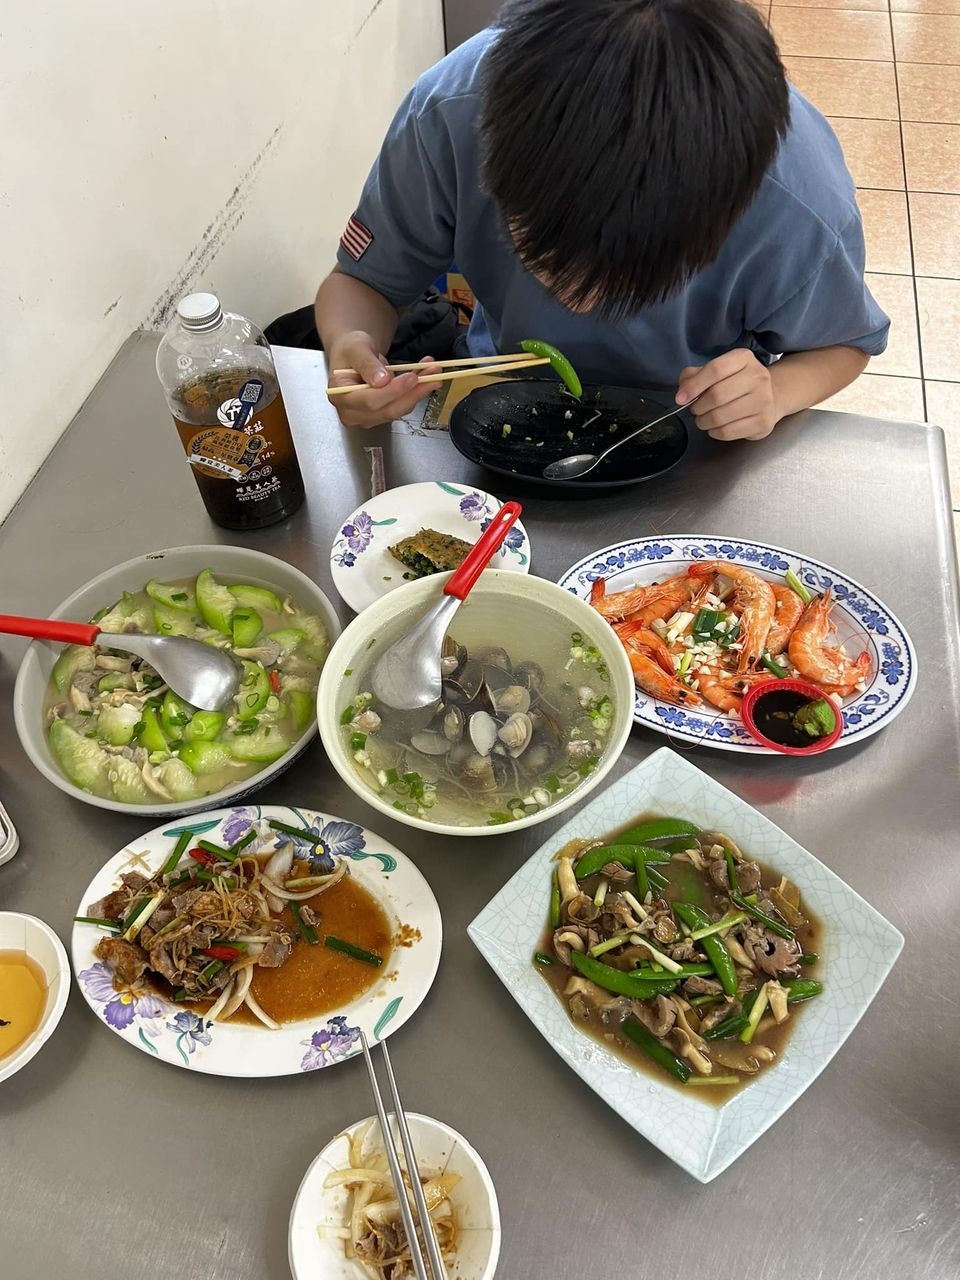
\includegraphics[width=\linewidth]{seafood.jpg}
  \end{tcolorbox}
  \begin{tcolorbox}[sidebyside, lefthand width=0.25\textwidth, colback=Violet!50!white, colframe=Violet]
    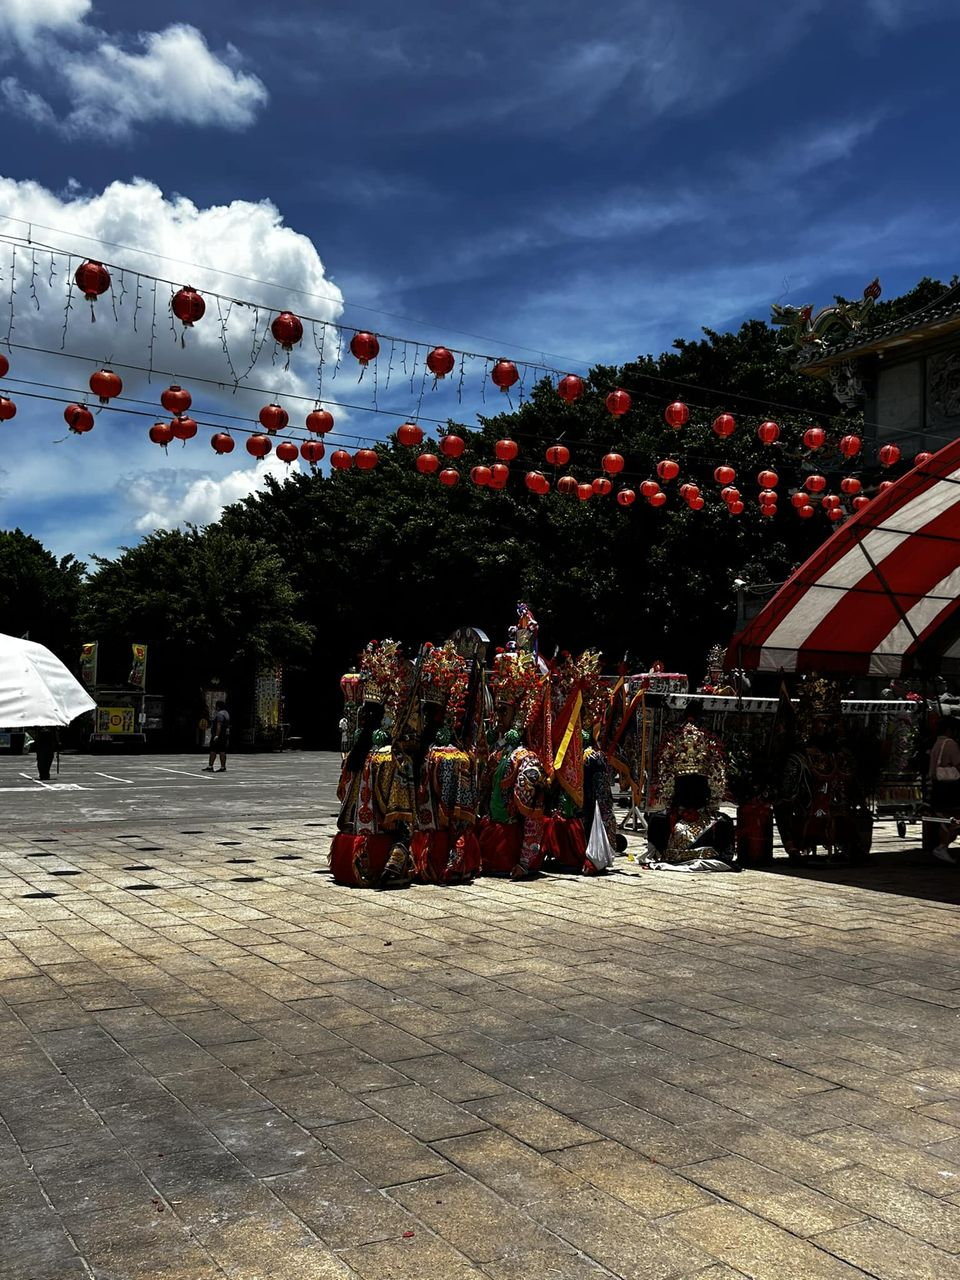
\includegraphics[width=\linewidth]{gods.jpg}
  \tcblower
  走出餐廳後,遇到了彰化當地的特殊儀式。據當地人所說,王功在 7/13 到 7/14
    耗時有舉辦漁火節,晚上還有煙火秀可以觀賞。雖然聽起來非常有趣,但因為還有接下來的形成無法久留,實在可惜。不過,廟會內的樂隊仍然令人心情鼓舞,離開時也沒有遺憾。
  \end{tcolorbox}
\end{boxpar}

    \begin{boxpar}{Violet}{第二站:嘉義旺來山}
        國中一年級時,去了嘉義旺來山的許願區許願自己考上好高中。到了三年後,我的確考上了第一志願:師大附中。雖然當時承諾會去還願,但因為時間的限制而無法這麼做。直到在這次暑假才有機會回訪旺來山。在這次旅程不但不食言地在旺來山還願,還許下新的願望:考上心中的理想台大電機系。
    \end{boxpar}
\begin{boxpar}{Violet}{第三站:台中雪山—稍來山}
  \begin{tcolorbox}[sidebyside, lefthand width=0.25\textwidth, colback=Violet!50!white, colframe=Violet]
    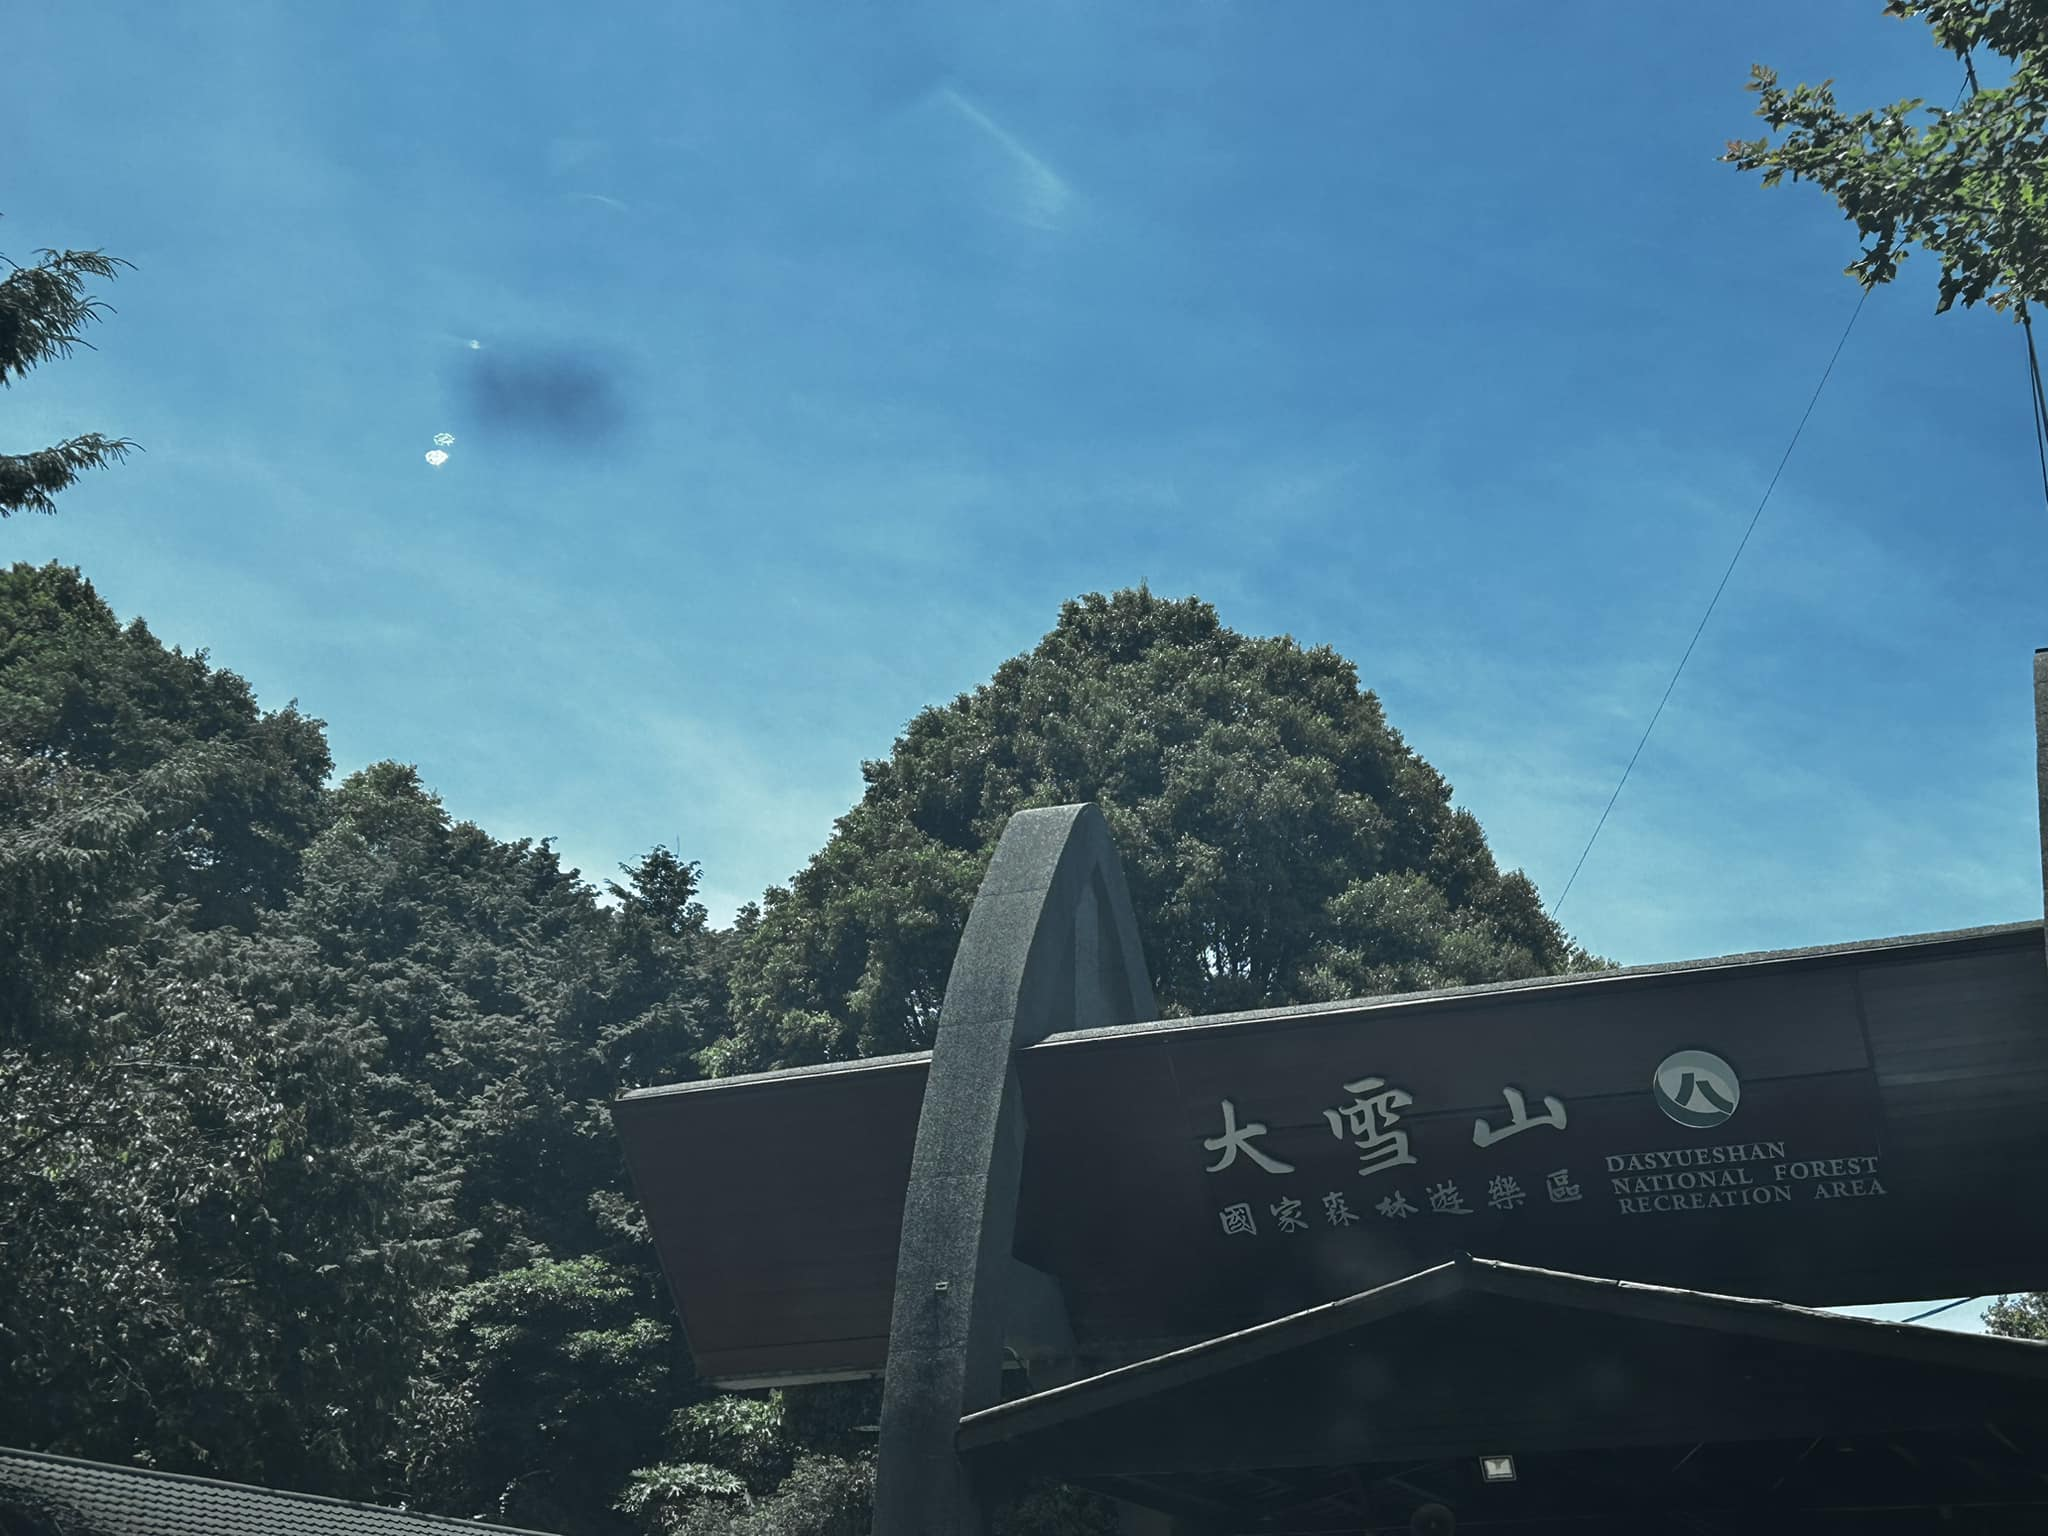
\includegraphics[width=\linewidth]{mountsnow.jpg}
    \tcblower
    稍來山是一座小百岳。當時去的時候繞了好一陣子的山路才到那邊。神奇的是,據說雪山國家公園為了讓垃圾不留山中而少有餐廳。換句話說遊客必須自己準備午餐,不然會在山上餓肚子。這件事情讓我大開眼界。\\

    吃完午餐上路後,赫然發現山林間安靜的像個圖書館,讓我們三位不速之客看起來格格不入。雖說是暑假,但山上竟然很少遇到其他山友更是讓這種寧靜的氣氛擴散到整座稍來山。
  \end{tcolorbox}
\end{boxpar}

\end{large}
\end{document}
